

% Gradient Info
  
\tikzset {_kdbe20a91/.code = {\pgfsetadditionalshadetransform{ \pgftransformshift{\pgfpoint{0 bp } { 0 bp }  }  \pgftransformrotate{-90 }  \pgftransformscale{2 }  }}}
\pgfdeclarehorizontalshading{_2uy0ym1vv}{150bp}{rgb(0bp)=(0.96,0.96,0.96);
rgb(43.30357142857143bp)=(0.96,0.96,0.96);
rgb(58.553292410714285bp)=(0.88,0.88,0.88);
rgb(100bp)=(0.88,0.88,0.88)}

% Gradient Info
  
\tikzset {_gma3lvhx6/.code = {\pgfsetadditionalshadetransform{ \pgftransformshift{\pgfpoint{0 bp } { 0 bp }  }  \pgftransformrotate{-90 }  \pgftransformscale{2 }  }}}
\pgfdeclarehorizontalshading{_ckay7h6o4}{150bp}{rgb(0bp)=(0.96,0.96,0.96);
rgb(43.30357142857143bp)=(0.96,0.96,0.96);
rgb(58.553292410714285bp)=(0.88,0.88,0.88);
rgb(100bp)=(0.88,0.88,0.88)}

% Gradient Info
  
\tikzset {_htck7z5md/.code = {\pgfsetadditionalshadetransform{ \pgftransformshift{\pgfpoint{0 bp } { 0 bp }  }  \pgftransformrotate{-90 }  \pgftransformscale{2 }  }}}
\pgfdeclarehorizontalshading{_a9lyv0hls}{150bp}{rgb(0bp)=(0.96,0.96,0.96);
rgb(43.30357142857143bp)=(0.96,0.96,0.96);
rgb(58.553292410714285bp)=(0.88,0.88,0.88);
rgb(100bp)=(0.88,0.88,0.88)}

% Gradient Info
  
\tikzset {_f0lkgujyf/.code = {\pgfsetadditionalshadetransform{ \pgftransformshift{\pgfpoint{0 bp } { 0 bp }  }  \pgftransformrotate{-90 }  \pgftransformscale{2 }  }}}
\pgfdeclarehorizontalshading{_e1ldk6rgh}{150bp}{rgb(0bp)=(0.96,0.96,0.96);
rgb(43.30357142857143bp)=(0.96,0.96,0.96);
rgb(58.553292410714285bp)=(0.88,0.88,0.88);
rgb(100bp)=(0.88,0.88,0.88)}

% Gradient Info
  
\tikzset {_h83ak7psv/.code = {\pgfsetadditionalshadetransform{ \pgftransformshift{\pgfpoint{0 bp } { 0 bp }  }  \pgftransformrotate{-90 }  \pgftransformscale{2 }  }}}
\pgfdeclarehorizontalshading{_7aeqfhyni}{150bp}{rgb(0bp)=(0.96,0.96,0.96);
rgb(43.30357142857143bp)=(0.96,0.96,0.96);
rgb(58.553292410714285bp)=(0.88,0.88,0.88);
rgb(100bp)=(0.88,0.88,0.88)}

% Gradient Info
  
\tikzset {_bzbwl9s0d/.code = {\pgfsetadditionalshadetransform{ \pgftransformshift{\pgfpoint{0 bp } { 0 bp }  }  \pgftransformrotate{-90 }  \pgftransformscale{2 }  }}}
\pgfdeclarehorizontalshading{_o4bxs07nh}{150bp}{rgb(0bp)=(0.96,0.96,0.96);
rgb(37.5bp)=(0.96,0.96,0.96);
rgb(50.982142857142854bp)=(0.87,0.87,0.89);
rgb(100bp)=(0.87,0.87,0.89)}
\tikzset{every picture/.style={line width=0.75pt}} %set default line width to 0.75pt        

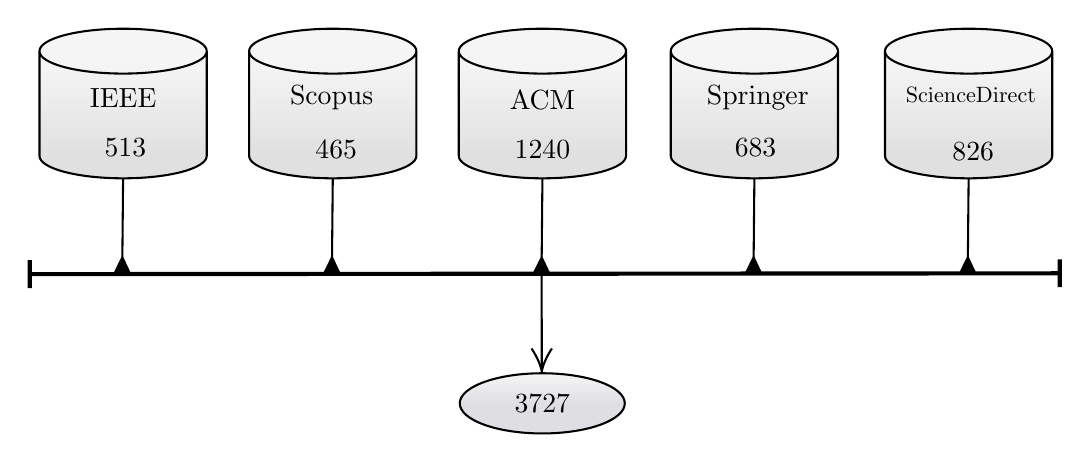
\begin{tikzpicture}[x=0.75pt,y=0.75pt,yscale=-1,xscale=1]
%uncomment if require: \path (0,421); %set diagram left start at 0, and has height of 421

%Shape: Can [id:dp367210882965306] 
\path  [shading=_2uy0ym1vv,_kdbe20a91] (581.45,74.81) -- (581.45,125.27) .. controls (581.45,131.24) and (563.41,136.08) .. (541.16,136.08) .. controls (518.9,136.08) and (500.86,131.24) .. (500.86,125.27) -- (500.86,74.81)(581.45,74.81) .. controls (581.45,80.78) and (563.41,85.62) .. (541.16,85.62) .. controls (518.9,85.62) and (500.86,80.78) .. (500.86,74.81) .. controls (500.86,68.84) and (518.9,64) .. (541.16,64) .. controls (563.41,64) and (581.45,68.84) .. (581.45,74.81) -- cycle ; % for fading 
 \draw   (581.45,74.81) -- (581.45,125.27) .. controls (581.45,131.24) and (563.41,136.08) .. (541.16,136.08) .. controls (518.9,136.08) and (500.86,131.24) .. (500.86,125.27) -- (500.86,74.81)(581.45,74.81) .. controls (581.45,80.78) and (563.41,85.62) .. (541.16,85.62) .. controls (518.9,85.62) and (500.86,80.78) .. (500.86,74.81) .. controls (500.86,68.84) and (518.9,64) .. (541.16,64) .. controls (563.41,64) and (581.45,68.84) .. (581.45,74.81) -- cycle ; % for border 

%Shape: Can [id:dp26297274922570457] 
\path  [shading=_ckay7h6o4,_gma3lvhx6] (478.23,74.81) -- (478.23,125.27) .. controls (478.23,131.24) and (460.19,136.08) .. (437.94,136.08) .. controls (415.68,136.08) and (397.64,131.24) .. (397.64,125.27) -- (397.64,74.81)(478.23,74.81) .. controls (478.23,80.78) and (460.19,85.62) .. (437.94,85.62) .. controls (415.68,85.62) and (397.64,80.78) .. (397.64,74.81) .. controls (397.64,68.84) and (415.68,64) .. (437.94,64) .. controls (460.19,64) and (478.23,68.84) .. (478.23,74.81) -- cycle ; % for fading 
 \draw   (478.23,74.81) -- (478.23,125.27) .. controls (478.23,131.24) and (460.19,136.08) .. (437.94,136.08) .. controls (415.68,136.08) and (397.64,131.24) .. (397.64,125.27) -- (397.64,74.81)(478.23,74.81) .. controls (478.23,80.78) and (460.19,85.62) .. (437.94,85.62) .. controls (415.68,85.62) and (397.64,80.78) .. (397.64,74.81) .. controls (397.64,68.84) and (415.68,64) .. (437.94,64) .. controls (460.19,64) and (478.23,68.84) .. (478.23,74.81) -- cycle ; % for border 

%Shape: Can [id:dp22020354780833284] 
\path  [shading=_a9lyv0hls,_htck7z5md] (376.11,74.81) -- (376.11,125.27) .. controls (376.11,131.24) and (358.07,136.08) .. (335.82,136.08) .. controls (313.56,136.08) and (295.52,131.24) .. (295.52,125.27) -- (295.52,74.81)(376.11,74.81) .. controls (376.11,80.78) and (358.07,85.62) .. (335.82,85.62) .. controls (313.56,85.62) and (295.52,80.78) .. (295.52,74.81) .. controls (295.52,68.84) and (313.56,64) .. (335.82,64) .. controls (358.07,64) and (376.11,68.84) .. (376.11,74.81) -- cycle ; % for fading 
 \draw   (376.11,74.81) -- (376.11,125.27) .. controls (376.11,131.24) and (358.07,136.08) .. (335.82,136.08) .. controls (313.56,136.08) and (295.52,131.24) .. (295.52,125.27) -- (295.52,74.81)(376.11,74.81) .. controls (376.11,80.78) and (358.07,85.62) .. (335.82,85.62) .. controls (313.56,85.62) and (295.52,80.78) .. (295.52,74.81) .. controls (295.52,68.84) and (313.56,64) .. (335.82,64) .. controls (358.07,64) and (376.11,68.84) .. (376.11,74.81) -- cycle ; % for border 

%Shape: Can [id:dp47910417750400036] 
\path  [shading=_e1ldk6rgh,_f0lkgujyf] (275.1,74.81) -- (275.1,125.27) .. controls (275.1,131.24) and (257.06,136.08) .. (234.81,136.08) .. controls (212.55,136.08) and (194.51,131.24) .. (194.51,125.27) -- (194.51,74.81)(275.1,74.81) .. controls (275.1,80.78) and (257.06,85.62) .. (234.81,85.62) .. controls (212.55,85.62) and (194.51,80.78) .. (194.51,74.81) .. controls (194.51,68.84) and (212.55,64) .. (234.81,64) .. controls (257.06,64) and (275.1,68.84) .. (275.1,74.81) -- cycle ; % for fading 
 \draw   (275.1,74.81) -- (275.1,125.27) .. controls (275.1,131.24) and (257.06,136.08) .. (234.81,136.08) .. controls (212.55,136.08) and (194.51,131.24) .. (194.51,125.27) -- (194.51,74.81)(275.1,74.81) .. controls (275.1,80.78) and (257.06,85.62) .. (234.81,85.62) .. controls (212.55,85.62) and (194.51,80.78) .. (194.51,74.81) .. controls (194.51,68.84) and (212.55,64) .. (234.81,64) .. controls (257.06,64) and (275.1,68.84) .. (275.1,74.81) -- cycle ; % for border 

%Shape: Can [id:dp2245173518314696] 
\path  [shading=_7aeqfhyni,_h83ak7psv] (174.09,74.81) -- (174.09,125.27) .. controls (174.09,131.24) and (156.05,136.08) .. (133.79,136.08) .. controls (111.54,136.08) and (93.5,131.24) .. (93.5,125.27) -- (93.5,74.81)(174.09,74.81) .. controls (174.09,80.78) and (156.05,85.62) .. (133.79,85.62) .. controls (111.54,85.62) and (93.5,80.78) .. (93.5,74.81) .. controls (93.5,68.84) and (111.54,64) .. (133.79,64) .. controls (156.05,64) and (174.09,68.84) .. (174.09,74.81) -- cycle ; % for fading 
 \draw   (174.09,74.81) -- (174.09,125.27) .. controls (174.09,131.24) and (156.05,136.08) .. (133.79,136.08) .. controls (111.54,136.08) and (93.5,131.24) .. (93.5,125.27) -- (93.5,74.81)(174.09,74.81) .. controls (174.09,80.78) and (156.05,85.62) .. (133.79,85.62) .. controls (111.54,85.62) and (93.5,80.78) .. (93.5,74.81) .. controls (93.5,68.84) and (111.54,64) .. (133.79,64) .. controls (156.05,64) and (174.09,68.84) .. (174.09,74.81) -- cycle ; % for border 

%Straight Lines [id:da8063181741938354] 
\draw [line width=1.5]    (88.82,182.25) -- (585.07,181.85) ;
\draw [shift={(585.07,181.85)}, rotate = 539.95] [color={rgb, 255:red, 0; green, 0; blue, 0 }  ][line width=1.5]    (0,6.71) -- (0,-6.71)   ;
\draw [shift={(88.82,182.25)}, rotate = 539.95] [color={rgb, 255:red, 0; green, 0; blue, 0 }  ][line width=1.5]    (0,6.71) -- (0,-6.71)   ;
%Straight Lines [id:da04659966611813071] 
\draw    (133.79,136.08) -- (133.43,174.05) ;
\draw [shift={(133.44,173.05)}, rotate = 90.54] [fill={rgb, 255:red, 0; green, 0; blue, 0 }  ][line width=0.75]  [draw opacity=0] (8.93,-4.29) -- (0,0) -- (8.93,4.29) -- cycle    ;

%Straight Lines [id:da7123071533494616] 
\draw [line width=0.75]    (335.45,183.05) -- (335.5,227) ;
\draw [shift={(335.5,229)}, rotate = 269.94] [color={rgb, 255:red, 0; green, 0; blue, 0 }  ][line width=0.75]    (10.93,-4.9) .. controls (6.95,-2.3) and (3.31,-0.67) .. (0,0) .. controls (3.31,0.67) and (6.95,2.3) .. (10.93,4.9)   ;

%Straight Lines [id:da037978733368861706] 
\draw    (234.81,136.08) -- (234.45,174.05) ;
\draw [shift={(234.46,173.05)}, rotate = 90.54] [fill={rgb, 255:red, 0; green, 0; blue, 0 }  ][line width=0.75]  [draw opacity=0] (8.93,-4.29) -- (0,0) -- (8.93,4.29) -- cycle    ;

%Straight Lines [id:da8972295671751513] 
\draw    (335.82,136.08) -- (335.46,174.05) ;
\draw [shift={(335.47,173.05)}, rotate = 90.54] [fill={rgb, 255:red, 0; green, 0; blue, 0 }  ][line width=0.75]  [draw opacity=0] (8.93,-4.29) -- (0,0) -- (8.93,4.29) -- cycle    ;

%Straight Lines [id:da1432985950729515] 
\draw    (437.94,136.08) -- (437.58,174.05) ;
\draw [shift={(437.58,173.05)}, rotate = 90.54] [fill={rgb, 255:red, 0; green, 0; blue, 0 }  ][line width=0.75]  [draw opacity=0] (8.93,-4.29) -- (0,0) -- (8.93,4.29) -- cycle    ;

%Straight Lines [id:da646269410198852] 
\draw    (541.16,136.08) -- (540.8,174.05) ;
\draw [shift={(540.8,173.05)}, rotate = 90.54] [fill={rgb, 255:red, 0; green, 0; blue, 0 }  ][line width=0.75]  [draw opacity=0] (8.93,-4.29) -- (0,0) -- (8.93,4.29) -- cycle    ;

%Shape: Ellipse [id:dp07212159007821795] 
\path  [shading=_o4bxs07nh,_bzbwl9s0d] (296,244.5) .. controls (296,236.49) and (313.8,230) .. (335.75,230) .. controls (357.7,230) and (375.5,236.49) .. (375.5,244.5) .. controls (375.5,252.51) and (357.7,259) .. (335.75,259) .. controls (313.8,259) and (296,252.51) .. (296,244.5) -- cycle ; % for fading 
 \draw   (296,244.5) .. controls (296,236.49) and (313.8,230) .. (335.75,230) .. controls (357.7,230) and (375.5,236.49) .. (375.5,244.5) .. controls (375.5,252.51) and (357.7,259) .. (335.75,259) .. controls (313.8,259) and (296,252.51) .. (296,244.5) -- cycle ; % for border 


% Text Node
\draw (133.79,97.23) node  [align=left] {IEEE};
% Text Node
\draw (234.25,97.23) node  [align=left] {Scopus};
% Text Node
\draw (335.82,98.13) node  [align=left] {ACM};
% Text Node
\draw (439.59,97.13) node  [align=left] {Springer};
% Text Node
\draw (542.26,96.02) node [scale=0.8] [align=left] {ScienceDirect};
% Text Node
\draw (134.9,121.19) node [scale=1] [align=left] {513};
% Text Node
\draw (236.46,122.09) node [scale=1] [align=left] {465};
% Text Node
\draw (335.82,122.09) node [scale=1] [align=left] {1240};
% Text Node
\draw (438.49,121.19) node [scale=1] [align=left] {683};
% Text Node
\draw (543.36,122.98) node [scale=1] [align=left] {826};
% Text Node
\draw (335.75,244.5) node  [align=left] {3727};


\end{tikzpicture}
